\chapter{A Conceptual Framework for Unsupervised Morphological Learning}
\label{ch:lit-review}

\section{Introduction}
\label{sec:framework-intro}
\cite{mccarthy:1981} points out a fundamental flaw in linear, 
concatenative approaches to morphological analysis: 
Such approaches acknowledge only a single level of representation, 
namely that of the \emph{segmental string}, i.e., the level of minimal 
phonological segments (essentially phonemes).\footnote{McCarthy uses
 the term \emph{segment} in the phonological sense, i.e., a minimal unit of sound. Researchers in unsupervised morphological learning, however, generally use the word to 
refer to minimal morphological units, 
as in \textit{the problem of morphological segmentation}, for example.}
Because they are restricted to this single layer, they can only represent 
morphological groupings in one way, namely to insert delimiters of 
some sort 
into the very string under analysis. At any given
insertion point, moreover, such an approach can see only two (phonological) segments, namely the one immediately to the left and the one immediately to the right.
It thus
has no way to identify morphs that are made up of discontiguous phonemes.

\cite{mccarthy:1981} offers an alternative \emph{nonlinear} 
approach to grouping segments into morphs, one that liberates the 
representation of morphs from the segmental tier. McCarthy's formalism, 
\emph{autosegmental morphology}, is an extension of the autosegmental 
approach to phonology developed by \citet{goldsmith:1976} to account 
for nonlinear phonological phenomena. One such phenomenon, for instance, 
is \emph{tone spreading}, whereby the tone on one vowel spreads to other 
vowels, leapfrogging any intervening consonants. 
Goldsmith's solution was to introduce \emph{autosegmental} tiers 
(or planes) of representation that were independent of and external 
to the segmental tier---tiers that could thus ``see'' and access any 
phonological segment in the segmental tier, as well as any subsequence 
of segments, contiguous or discontiguous. The key was the nonlinearity 
(or multilinearity)
introduced by the multiple tiers and their separation both from each other 
and the segmental tier. 
McCarthy's insight was that this same nonlinear architecture could be 
applied to the problem of nonconcatenative morphology, particularly the 
root-and-pattern morphology of Semitic languages. 

I have devised a framework for comparing (and classifying)
previous approaches
the unsupervised learning of morphology. This framework is a classification 
system derived from the definitions of nonlinearity and nonsequentiality 
(see chapter~\ref{ch:intro}, definitions \ref{def:nl} and \ref{def:ns}) 
and the proposition that 
a model can learn nonconcatenative morphology if and only if it 
possesses both of these categories (chapter~\ref{ch:intro}, 
proposition~\ref{prop:nlns}). In particular, first observe that nonlinearity 
and nonsequentiality are negative concepts and thus suggest the existence 
of their positive counterparts, \emph{linearity} and 
\emph{sequentiality}. To facilitate the exposition of these concepts, we 
repeat the definitions of nonlinearity and nonsequentiality here and 
then define their complements, \emph{linearity} and \emph{sequentiality}.
\smallskip
	\begin{description}[itemsep=2pt]
	%\begin{definition*}
	\item[Nonlinearity:]A model is 
	\textbf{nonlinear} if each of its morphs occupies a tier that is \emph{not} the phonological tier.
	%\end{definition*}
	%\begin{definition*}
	%\label{def:ns}
	\item[Nonsequentiality:]
	A model is \textbf{nonsequential} if \textbf{no two morphs} occupy the \emph{same} tier. This is to say that all morphs are independent, i.e., there are no morph-to-morph connections. 
	\end{description}
	\smallskip
	\begin{definition}\label{def:l}{\textbf{Linearity}}:
	A model is \textbf{linear} if at least some of its morphs occupy the phonological tier.
	\end{definition}
	\begin{definition}\label{def:s}{\textbf{Sequentiality}}:
A model is \textbf{sequential} if two or more morphs occupy the \emph{same} tier.\footnote{In practice, `` two or more morphs'' is tantamount to saying ``all morphs,'' since it is hard to envision a scenario in which only a subset of morphs occupy their own tiers.} This is to say that there are connections between at least some pairs of morphs.
	\end{definition}
	\medskip
	\vspace{4pt}
Proposition~\ref{prop:nlns} in chapter~\ref{ch:intro} conditions an algorithm's ability to model nonconcatenative morphology on the \emph{conjunction} of nonlinearity and nonsequentiality. That is, 
\smallskip
\begin{quote}\noindent
A model of morphology can represent nonconcatenative morphology if it is nonlinear \emph{and} nonsequential.
\end{quote}
\smallskip
Thus, the desired category is the \emph{intersection} of the basic nonlinear and nonsequential categories, and because it is the desired category, it has to be a category in our conceptual framework.
%It stands to reason that the other categories would be related to this desired category. In par
The other categories are similarly derived by taking pairwise intersections of the basic categories outlined above, as shown in figure~\ref{fig:intersections}.
The resulting framework thus consists of two orthogonal axes, each representing one of two binary distinctions,
namely ``linear vs. nonlinear'' and ``sequential vs. nonsequential." The following sections will discuss each of these categories
in turn, citing examples 
for each. 
\begin{figure}[!h]
\centering
\fbox{\begin{minipage}{9cm}
\centering
\textbf{Nonlinear-nonsequential} $=$ nonlinear $\cap$ nonsequential \\
\textbf{Nonlinear-sequential} $=$ nonlinear $\cap$ sequential \\
\textbf{Linear-nonsequential} $=$ linear $\cap$ nonsequential \\
\textbf{Linear-sequential} $=$ linear $\cap$ sequential
\end{minipage}}
\label{fig:intersections}
\caption{Four-category framework}
\end{figure}
%will use the term
%\textbf{nonlinear} (NL) to refer to learning
%models (or algorithms) one
%or more hidden layers to encode the
%morphological structure.
%We use the term \emph{nonlinear} in the sense of \citep{mccarthy:1981, goldsmith:1976}, i.e., 
%to describe learning models that incorporate more than one tier of representation, i.e., more than 
%just the words (segmental strings) themselves.
%Proposition \ref{prop:nlns} asserts that \emph{both} nonlinearity \emph{and} nonsequentiality
%must be present in a model if it is to capable of modeling nonconcatenative morphology.
%A model of morphology can represent nonconcatenative morphology if it is nonlinear and nonsequential.
% In other words, the category of models capable of the learning nonconcatenative 
% morphology is  the intersection of the (more general) nonlinear and 
% sequential categories. Thus, one of our framework's categories has to be 
% \textbf{nonlinear-nonsequential}. Indeed, this is the ``desired'' category, 
% so to speak, the category whose members are intrinsically capable of modeling/learning
% nonconcatenative morphology. 
 
% The other categories are likewise intersections
% of the basic categories outlined above.  They are derived as follows: 
% 
% For instance, another category is \textbf{nonlinear-sequential}, 
% or the intersection of the nonlinear and sequential categories. The remaining two categories, 
% \textbf{linear-nonsequential} and \textbf{linear-sequential} are analogously defined. The four categories are summarized in figure~\ref{fig:intersections}:



%\fbox{\begin{minipage}{9cm}
%\centering
%\textbf{Nonlinear-nonsequential} $=$ nonlinear $\cap$ nonsequential \\
%\textbf{Nonlinear-sequential} $=$ nonlinear $\cap$ sequential \\
%\textbf{Linear-nonsequential} $=$ linear $\cap$ nonsequential \\
%\textbf{Linear-sequential} $=$ linear $\cap$ sequential
%\end{minipage}}

% derived from the concepts \emph{nonlinearity} and 
%\emph{nonsequentiality}  and their respective complements 
%\emph{linearity} and \emph{sequentiality}. 
% We can think of the terms \emph{nonlinear} and \emph{nonsequential} as labels 
%for basic categories of models, namely the those that have the 
%property \emph{nonlinearity} and those that have the property 
%\emph{nonsequentiality}, respectively. Recall proposition \ref{prop:nlns}, 
%which posits that \emph{both} nonlinearity and nonsequentiality must be 
%present in a model if it is to be able to handle nonconcatenative morphology. 
%In other words, a model must belong to the \emph{intersection} of the 
%nonlinear and nonsequential models; i.e., it must be a \textbf{nonlinear nonsequential} 
%model.  And indeed, ``nonlinear-nonsequential'' is one of the categories of our four-category 
%framework.  The other three are derived similarly:
 

%In particular, the ``negative'' properties \emph{nonlinearity} and \emph{nonsequentiality} 
%imply the existence of their ``positive'' counterparts, namely  \emph{linearity} and \emph{sequentiality}, respectively, which correspond to the basic-category labels \emph{linear} and \emph{sequential}. We thus define
%\emph{linearity} and \emph{sequentiality} as the opposites of \emph{nonlinearity} and \emph{nonsequentiality}, respectively.
%
%	\begin{definition}\label{def:l}{\textsc{Linearity}}: %A model is \emph{nonlinear} 
%	Morphs are \emph{not} separate from the phonological tier. \end{definition}
%	\begin{definition}\label{def:s}{\textsc{Sequentiality}}:
%	Not all morph tiers are orthogonal to the other morph tiers
%	\end{definition}
% Proposition \ref{prop:nlns} states that \textbf{nonlinear nonsequential} needs to be one of framework's categories, and it is obtained by taking the intersection of the basic categories \emph{nonlinear} and \emph{nonsequential}. We derive the other categories by taking analogous intersections of basic categories, as follows:
%\begin{itemize}
%\item \textbf{Nonlinear-nonsequential} $=$ nonlinear $\cap$ nonsequential
%\item \textbf{Nonlinear-sequential} $=$ nonlinear $\cap$ sequential
%\item \textbf{Linear-nonsequential} $=$ linear $\cap$ nonsequential
%\item \textbf{{Linear-sequential} $=$ linear $\cap$ sequential
%\end{itemize}
%The linear-sequential category is the intersection of the linear and sequential basic categories; the nonlinear-sequential category is 

%The resulting framework thus consists of two orthogonal axes, each representing one of two binary distinctions,
%namely ``linear vs. nonlinear'' and ``sequential vs. nonsequential." 
%We use the term \emph{nonlinear} in the sense of \citep{mccarthy:1981, goldsmith:1976}, i.e., 
%to describe learning models that incorporate more than one tier of representation, i.e., more than 
%just the words (segmental strings) themselves.

%We thus use the term \emph{linear} in the sense of `one-dimensional' (i.e., in opposition to \emph{nonlinear}). 
%In particular, we use it to label learning models that  I in the sense that opposes our sense of nonlinear, i.e., 
%opposing categories to a pair of opposing categories; the first is learning models along two 
%orthogonal axes consists of four categories, namely  in two pairs of opposing categories, namely 
%``linear vs. nonlinear" and ``sequential vs. nonsequential." 
%We cross-combine these categories 
%to create a $2\times2$ grid, the cells of which represent create a total of four categories. 
%The first is the``linear vs. nonlinear" distinction of \citep{mccarthy:1981, goldsmith:1976} 
%to categorizing existing approaches in \ac{ULM}.


% in the
%surface layer, whereas 
%, the layer of the graphemes/phonemes.
% Here, \textit{hidden layer} is conceptually related to McCarthy's
% \textit{autosegmental tier}, but the two terms are not necessarily
% equivalent formally.  
%The term 
%\textbf{linear} (L), i.e., \emph{linear} in the sense of `one %(cf. ``one-dimensional'') 
%will serve as the label for 
%algorithms that operate solely within the layer of surface symbols.  %s the attempt to construct a representation of
%%morphological structure. 
%Typically, such algorithms denote the morph boundaries by inserting delimiters directly into segmental strings.
 %surface string with morpheme boundary symbols. %Note that we will be using \textit{linear} in the sense of `one dimensional,' rather than`in/like a (straight) line.'
% This definition is not unlike ``one dimensional," a fairly common
% sense of \textit{linear}.  We do not, however, use \textit{linear} to
% mean ``in/like a straight line."
%but one to be distinguished from ``in/like a straight line." As it is used in this paper, the term \textit{linear} s not related in any direct way to the notions of line and straightness.
%We do not, however, use \textit{linear} to mean ``in a straight line" or even ``like a straight line."
%

%In addition to the 
%\textit{linear} vs. {nonlinear} distinction, we will also introduce a distinction between each into
%\textbf{sequential} and \textbf{nonsequential}.
%%, obtaining four categories in all. We describe each below.
%An algorithm is sequential (S) if there is a necessary sequence to its morphological classification decisions, i.e., if, for any two decisions, one must precede the other.\footnote{By \textit{morphological 
%%if its makes morphological classification decisions depend on preceding or succeeding context, i.e., if there is a necessary sequence to its decisions.
%%presentational unit (or feature) depends on the immediately preceding unit(s). %the value of each representational unit is determined independently of all other units
%classification decision}, we mean any decision that maps an atomic representational unit (usually a character or a feature) to a morphological category. This definition includes simple ``split" decisions, where there are only two possible categories: ``part of the current morpheme" and ``part of the next morpheme."}
%On the other hand, in a nonsequential (NS) algorithm, all morphological classification decisions are made in parallel; i.e., the decisions are unordered.
%
% We thus have a total of four categories: linear sequential (LS),
% linear nonsequential  (LNS), non-linear sequential  (NLS), and finally
% nonsequential nonlinear (NLNS). In what follows, we describe each of these in turn.

%We will now discuss and exemplify each of these categories in turn.

%\section{linear sequential algorithms}
%\label{subsec:seq-lin}
%
%The linear sequential (LS) type of algorithm is depicted in figure~\ref{fig:seq-lin}. 
%LS algorithms consider only one layer of representation, namely the surface layer. They use no hidden layers, hence their linearity. The surface layer is made up of surface units, depicted as squares in figure~\ref{fig:seq-lin}.
%In LS algorithms, these squares are usually the characters themselves. 
%The task is to assign each character to a morphological class. Thus, in effect, 
%each square represents a morphological classification decision.
%The arrows indicate the sequential order of the algorithm's decisions. 
%The fact that there is such an order is the reason this type of algorithm is sequential.
%
%The first unsupervised morphological learners were LS algorithms. The earliest examples employed the Letter Successor/Predecessor Variety (LSV/LPV) measures \citep{harris:1955, harris:1967}. 
%Both measures are intended to indicate likely affixes.
%$\text{LSV}(x)$ is intended to find prefixes; given a string $x$ and corpus $W$, $\text{LSV}(x)$ returns the number of letter types that immediately follow $x$ whenever $x$ is word-initial in $W$.
%Letter Predecessor Variety (LPV) is essentially the same measure, except that its function is to find suffixes:
%%That is, LPV is simply LSV from the opposite direction: 
%It counts the grapheme types that immediately \emph{precede} $x$ whenever $x$ is \emph{word-final}.
%%$\text{LSV}(x,W)$ is used to find prefix-stem boundaries, and $\text{LPV}(x)$ to find stem-suffix boundaries. 
%
%% Stress sequential nature of algorithm
%By themselves, of course, LSV and LSP are merely counts; they must be ``unpacked" if they are to be used to discover legitimate morpheme boundaries.
%There are a few different techniques for doing this
%%using LSV/LSP to discover morpheme boundaries 
%\citep[see][]{hammarstrom:2011}; one is the ``peak and plateau" technique. The following describes the use of peak and plateau with LSV: 
%
%\begin{itemize}
%\item Given an $n$-length word $w$ whose graphemes are indexed from 0 to $n$, compute $\text{LSV}(w[0:i])$ for each $i$ in the range $[0, n)$.
%%in the range $[0, n)$. 
%\item Then, for each $i$ in $[0, n)$, insert a morpheme boundary after the substring $w[0:i]$ if and only if 
%\begin{equation*}
%\text{LSV}(w[0:i-1]) \le \text{LSV}(w[0:i]) \ge \text{LSV}(w[0:i+1]),
%\end{equation*}
%i.e., there is a local peak in the LSV sequence at index $i$.
%\end{itemize}
%
%It is not difficult to see the sequentiality and linearity of an LSV/LPV technique like peak and plateau.
%Such a technique is sequential because its decision making process is shaped by the sequential order of graphemes.
%An LSV technique, for example, must proceed left to right, one index at a time, because the LSV calculation at index $i$ depends on the preceding $i-1$ graphemes. Moreover, in peak and plateau, the question of whether or not to draw a morpheme boundary at index $i$ depends not only on the LSV at $i$, but also on the preceding and succeeding LSVs. LSV/LPV techniques are linear because they incorporate no hidden nodes and thus have no means of mediating associations between nonadjacent characters.
%
%The intuition behind the LSV/LPV method is that \emph{within} a morpheme, the identity of each letter depends on the letters that immediately precede or succeed it. But this is not the case \emph{between} morphemes. That is, the first letter of a morpheme is largely unpredictable given its preceding letters. Likewise, a morpheme's final letter is largely unpredictable given its succeeding letters. Thus, the number
% of possible letter types tends to increase sharply at the boundary between two morphemes.
%
%However, while morpheme boundaries generally coincide with high LVP/LSV counts, it is not necessarily true that a high LVP/LSV indicates a morpheme boundary.
%%LSV is not always a reliable indicator of morpheme boundaries. 
%\cite{hammarstrom:2011}, for example, provide LPV counts for the word \textit{disturbance}. 
%The highest LPV count of 25 
%%(i.e., 25 of the 26 possible letters in the English alphabet) 
%occurs between \textit{disturbanc} and \textit{e}.
%An LPV-based analysis would thus incorrectly identify \textit{e} as a suffix, a consequence of the ubiquity of \textit{e} as a stem-final letter in English spelling. 
%
%%Goldsmith
%Because of such problems, most linear sequential methods today have abandoned LSV/LPV, often in favor of frequency-based heuristics.
%\cite{goldsmith:2001}, for example, uses a score based on pointwise mutual information (PMI) to approximate the likelihood that a given character $n$-gram $c_{1}c_{2}...c_{n}$ is a morpheme. 
%%In particular, the PMI of the characters $c_{1}, c_{2}, ..., c_{n}$ is multiplied by the relative frequency of the $n$-gram $c_{1}c_{2}...c_{n}$. 
%\cite{goldsmith:2001} obtains candidate suffixes (intended for further processing) by taking the $n$-grams that are ranked highest according to this score.  
%%(i.e., the count of $c_{1}c_{2}...c_{n}$ divided by the total count of all $n$-grams). 
%
%%Moon
%\cite{moon-et-al:2009} apply tree data structures known as \textit{tries} to the task of finding stems and affixes, as have a number of other researchers \citep[e.g.,][]{schone-and-jurafsky:2000, monson:2004, argamon:2004}.
%Tries are useful for learning concatenative morphology because they compactly store recurring character sequences.
%%that are repeated a group of words. by sets of words beginning with the same character. 
%Each node in a trie represents a certain prefix string (with the root node representing the empty string), 
%and every path proceeding out from a node represents a possible succeeding character. 
%Thus, even though tries are tree data structures, they process data in a sequential manner. 
%They 
%%also represent morphological relationships linearly 
%are linear
%because they lack hidden nodes, and every path through a trie is deterministic. 
% \cite{moon-et-al:2009} depart from other trie-based methods in using document 
% boundaries to approximate semantic context. 
% This helps them weed out spurious analyses like the \textit{disturbanc}+\textit{e} 
% example above, but it does not change the fundamentally sequential and linear nature of their approach.
%%\citep{goldsmith:2001} or trie-based affix-finding
%%\citep{moon-et-al:2009}.
%% , for example, uses a score based on pointwise mutual information
%% (PMI) to approximate the likelihood that a given character $n$-gram
%% %$c_{1}c_{2}...c_{n}$ 
%% is a morphemic unit.
%% In particular, the PMI of the characters $c_{1},
%% c_{2}, ..., c_{n}$ is multiplied by the relative frequency of the
%% $n$-gram $c_{1}c_{2}...c_{n}$. \cite{goldsmith:2001} obtains candidate
%% suffixes by taking the $n$-grams that are ranked highest according to
%% this score.
%%(i.e., the count of $c_{1}c_{2}...c_{n}$ divided by the total count of all $n$-grams).  
%%
%%Moon
%% \cite{moon-et-al:2009} apply tries to the task of finding stems and
%% affixes, to store recurring character sequences.
%%, as have a number of other researchers. 
%% Tries are useful for learning concatenative morphology because they
%% compactly store recurring character sequences.
%%that are repeated a group of words. by sets of words beginning with the same character. 
%% Each node in a trie represents a certain prefix string (with the root node representing the empty string), 
%% and every path proceeding out from a node represents a possible succeeding character. 
%% Thus, even though tries are tree data structures, 
%%In all cases, the methods process data in a sequential manner and
%%lack hidden nodes for representing morphological relationships.
%% linearly, lacking hidden nodes.
%
%% ; one of them is the ``peak and plateau" technique, which works as follows:
%% \begin{itemize}
%% \item Given an $n$-length word $w$ whose graphemes are indexed from 0 to $n$, compute $\text{LSV}(w[0:i])$ for each $i$ in the range $[0, n)$. \item Insert a morpheme boundary after the substring $w[0:i]$ if and only if $\text{LSV}(w[0:i-1]) \le \text{LSV}(w[0:i]) \ge \text{LSV}(w[0:i+1])$, i.e., there is a local peak in the LSV sequence at index $i$.
%% \end{itemize}
%% Notice the sequential nature of this technique: each LSV calculation is determined solely by the immediately preceding string of graphemes. Note also its linearity: there is only a single layer of representation for both the grapheme sequence and the morphological analysis.
%
% \begin{figure}[tb]
% %\begin{minipage}{.3\textwidth}
% \begin{center}
% \begin{tikzpicture}[shorten >=1pt,->,draw=black!100,node distance = 1.3cm, auto]]
% 	\def \startnode{1.5cm}
% %	\def\secondrow{1.0cm}
% 	\tikzstyle{r-node}=[regular polygon sides=4,draw=black!100,thick,inner sep=0pt,minimum size=4mm]
% 	\tikzstyle{annot} = [text width=3cm]
% %	\tikzstyle{annot} = [text width=2.0cm, text centered]
% 	% labels
% %	\node[annot] (m-label) at (0,\thirdrow) {hidden-unit vector};
% %	\node[annot] (r-label) at (0, \secondrow) {prediction vector};
% %	\node[annot] (d-label) (0, 0) {observed data vector};
% 	% hidden layer
% 	\node[annot] (surface-label) at (0cm,0cm) {surface layer};
% %	\node[annot] (r-label) at (0, \secondrow) {prediction vector};
% %	\node[annot] (d-label) (0, 0) {observed data vector};
%	
% 	% surface layer
% 	\node[r-node] 	(r0)	at (\startnode,0cm)		{};
% 	\node[r-node] 	(r1)	at (2.5cm, 0cm)		{};
% 	\node[r-node] 	(r2)	at (3.5cm,0cm)	 	{};
% 	\node[r-node] 	(r3)	at (4.5cm,0cm) 		{};
% 	\node[r-node] 	(r4) 	at (5.5cm,0cm)   		{};
%	
% 	\path (r0)	edge	node	{}	(r1)
% 		(r1)	edge	node	{}	(r2)
% 		(r2)	edge	node	{}	(r3)
% 		(r3)	edge	node	{}	(r4);
% \end{tikzpicture}
% \end{center}
% \caption{linear sequential architecture.}
% %. Each representational unit depends on the preceding unit, and no unit exists outside of the surface layer.}
% \label{fig:seq-lin}
% \end{figure}
%
%% The intuition behind the LSV/LPV method is related to that behind the entropy-based methods in natural language processing:
%% %In fact, LSV generally increases/decreases as entropy increases/deceases: 
%% At any given point \emph{within} a morpheme, the next letter is fairly predictable, which generally coincides with a smaller number of succeeding letter types. But at the border between two morphemes, the next letter is much less predictable. This low predictability generally translates to a much larger set of options for the succeeding letter (i.e., a higher LSV). However, it out that LSV is not always a reliable indicator of morpheme boundaries. \cite{hammarstrom:2011}, for example, provide LPV counts for the word \textit{disturbance}. 
%% The highest count (25) 
%% %(i.e., 25 of the 26 possible letters in the English alphabet) 
%% occurs between \textit{disturbanc} and \textit{e}, An LPV-based analysis would thus yield an incorrect result in this case, a consequence of the fact that \textit{e} is such a ubiquitous word-final letter in English spelling. 
%
%%Goldsmith
%% More recent linear sequential methods
%% %have thus abandoned LSV/LPV, often in favor of
%% use frequency-based heuristics.  \cite{goldsmith:2001}, for example,
%% uses a score based on pointwise mutual information (PMI) to
%% approximate the likelihood that a given character $n$-gram
%% %$c_{1}c_{2}...c_{n}$ 
%% is a morphemic unit.
%% % In particular, the PMI of the characters $c_{1},
%% % c_{2}, ..., c_{n}$ is multiplied by the relative frequency of the
%% % $n$-gram $c_{1}c_{2}...c_{n}$. \cite{goldsmith:2001} obtains candidate
%% % suffixes by taking the $n$-grams that are ranked highest according to
%% % this score.
%% %(i.e., the count of $c_{1}c_{2}...c_{n}$ divided by the total count of all $n$-grams).  
%% %
%% %Moon
%% \cite{moon-et-al:2009} applies \textit{tries} to the task of finding stems and
%% affixes, to store recurring character sequences in the search for recurring character sequences.
%% % A number of other researchers have done the same.
%% % Tries are useful for learning concatenative morphology because they
%% % compactly store recurring character sequences.
%% %that are repeated a group of words. by sets of words beginning with the same character. 
%% % Each node in a trie represents a certain prefix string (with the root node representing the empty string), 
%% % and every path proceeding out from a node represents a possible succeeding character. 
%% % Thus, even though tries are tree data structures, 
%% In all cases, the methods process data in a sequential manner and
%% represent morphological relationships linearly, lacking hidden nodes.
%
%% , and every path through a trie is deterministic.
%% \cite{moon-et-al:2009} depart from other trie-based methods in using
%% document boundaries to approximate semantic context.  This helps them
%% weed out spurious analyses like the \textit{disturbanc}+\textit{e}
%% example above, but it does not change the fundamentally sequential and
%% linear nature of their approach.
%
%\section{Linear nonsequential algorithms}
%\label{subsec:nonseq-lin}
%In the linear nonsequential (LNS) type of algorithm, shown in figure~\ref{fig:nonseq-lin}, the representational units are generally not raw characters, but rather \emph{features}, i.e., binary variables representing the presence or absence of particular properties.
%%specifying whether or not a word has a certain property. 
%Features in nonsequential algorithms need not correspond to contiguous chunks of the original string; for example, features like the following are perfectly valid: ``\textit{t} precedes \textit{i} within $\delta$ characters" and ``\textit{t} precedes \textit{b} within $\delta$ characters," where the character pairs \emph{t..i} and \emph{t..b} are discontiguous as long as $\delta \ne 0$. Notice that such features cannot really be ordered; each is either \textsc{true} or \textsc{false} irrespective of order.
%All nonsequential algorithms---of which LNS algorithms are a subcategory---view a given word's features as being unordered, i.e., as being sequentially unrelated to each other. 
%But while LNS algorithms are nonsequential, they are linear because they incorporate no hidden units. Thus, even though an LNS algorithm's features may refer to discontiguous subsequences of characters, they are nonetheless restricted to representing only properties that are overtly present in the surface layer of characters. 
%
%One LNS example is the algorithm of \cite{poon-et-al:2009}, which uses log-linear models to induce morphological segmentations for Arabic and Hebrew. 
%Log-linear models are inherently nonsequential because they treat all features as independent, estimating a global joint probability for the entire bag of features. 
%%Sequential models, in contrast, estimate conditional probabilities based on sequential dependencies between features
%The algorithm of \cite{poon-et-al:2009} in particular searches for the set of parameters $\theta$ that maximizes the joint probability of a corpus $W$ and a morphological segmentation $S$, i.e., $P(W,S| \theta) = P(W|S; \theta) \cdot P(S| \theta)$. The segmentation $S$ is encoded by a set of features.
%%They generate candidate segmentations via Gibbs sampling. For each candidate, they extract a feature set
%
%%Log-linear models are well-suited for large numbers of arbitrarily defined features. 
%\cite{poon-et-al:2009} use two categories of features to encode a morphological segmentation: \textit{morpheme features} and \textit{morpheme context} features.
%The former encode (potential) morpheme types and their frequencies, e.g., \texttt{vlAv:5} and \texttt{w:31}. The 
%latter encode context types and their frequencies, where a \emph{context} consists of the $n$ characters preceding and succeeding a (potential) morpheme;
%%the character bigrams to the left and right of a potential morpheme, 
%e.g., the feature \texttt{\#w\_wn:12} would represent a context whose left side consists of \textit{w} preceded by the word boundary, whose right side is the bigram \textit{wn}, and whose frequency is 12. Importantly, these context features overlap. That is, in \texttt{\#w\_wn:12}, the \textit{w} and \textit{wn} are themselves morphemes whose contexts must be extracted.
%This feature overlap is made possible by the nonsequentiality of log-linear models.
%%is on the right, , respectively, and whose frequency of this particular context as 12.
%%s that the left context is the character \textit{w} preceded by the word boundary, the right context is the character bigram \textit{wn}, and the frequency of this particular context is 12).
%% and \textand the characters \textit{w} and \textit{n} are on the right potential morpheme\textit{w} on the left 
%%and the characters \textit{w} and \textit{n} on the right).
%%Note, however, that 
%
%Note, however, that log-linear models can handle much more nonsequentiality than this. Indeed, since a log-linear models is inherently nonsequential, it accommodate any sort of nonsequential feature. 
%%one can incorporate into log-linear model.
%%feature %or combination of feature types 
%%in a log-linear model.  
%One could, for example, incorporate
%features representing discontiguous bigrams,
%as already noted.
% One could also combine contiguous and discontiguous bigram features in the same feature set.
%%for example, have features representing both contiguous and discontinous bigrams in the same feature set.
%%However, one in principle could use any sort of feature in a log linear model, such as a feature type representing discontiguous bigrams, for example.
%%Each feature represents the both corpus and the segmentation jointly, and a fully specified set of features thus represents an entire segmented corpus;
%%but there is no limit on the variety or quantity of features one can incorporate into a log-linear model.
%% Why is a log linear model nonsequential?
%%Log-linear models are inherently nonsequential because they treat all features as independent, estimating a global joint probability for the entire bag of features. Sequential models, in contrast, estimate conditional probabilities based on sequential dependencies between features.
%% Why is a log linear model nonsequential?
%And yet it is not the nature of the features themselves that makes an algorithm nonsequential, but rather the lack of sequential relationships between features. The algorithm of \cite{poon-et-al:2009} is nonsequential because it does not process features in a particular order.
%% Why is Poon et al's algorithm linear?
%It is, however, linear because it incorporates no hidden units to mediate associations between features.
%
%%\cite{poon-et-al:2009} incorporate no latent variables, however. 
%%Their representation of morphological structure makes reference only to the the surface layer of graphemes. Their morpheme features are limited to  contiguous grapheme sequences, 
%%and their morpheme context features encode only extreme left and right contexts, 
%%thus assuming no internal boundaries (i.e., no morpheme interruptions).
%%%They generate candidate segmentations via Gibbs sampling, but, for an $n$-length word, they consider 
%%Because it only acknowledges the surface layer of text, the algorithm of \cite{poon-et-al:2009} can only isolate stems and affixes, not the discontiguous roots and patterns of Arabic and Hebrew.
%
%%\paragraph{inear nonsequential algorithms}
%%\label{subsec:nonseq-lin}
%%
%%Like LS algorithms, \textbf{linear nonsequential } (LNS) algorithms consist only of surface units, having no hidden layer, hence their linearity. LNS algorithms are different in that there are no dependencies between representational units. Each unit is independent of other units, hence their \textit{nonsequential} characterization.
%%%They consist only of surface units, hence their linearity. What sets LNS algorithms apart is the lack of dependencies between these units, h
%%%illustrated in figure~\ref{fig:nonseq-lin}, 
%%%there are no dependencies between representational units, but also no
%%%hidden units.
%%%; i.e., all representational units reside in the surface layer.  
%%As one example, \cite{poon-et-al:2009} use log-linear models to induce
%%morphological segmentations for Arabic and Hebrew. 
%%% Their algorithm
%%% searches for the set of parameters $\theta$ that maximizes the joint
%%% probability of a corpus $W$ and a segmentation $S$ (i.e., $P(W,S|
%%% \theta)$).
%%% = P(W|S; \theta) \cdot P(S| \theta)$.
%%%They generate candidate segmentations via Gibbs sampling. For each candidate, they extract a feature set
%%% Log-linear models are well-suited for large numbers of arbitrarily
%%% defined features.
%%% \cite{poon-et-al:2009} use morpheme features and morpheme context
%%% features.  The former category specifies a morpheme type and its
%%% frequency, e.g., \texttt{vlav:1} and \texttt{w:2}.  The latter
%%% category indicates the character bigrams to the left and right of a
%%% given morpheme, e.g., \texttt{\#w\_wn:1} (a word boundary followed by
%%% the character \textit{w} on the left and the characters \textit{w} and
%%% \textit{n} on the right).  Note, however, that one could use any type
%%% of feature or combination of feature types with a log-linear
%%% model. One could, for example, have features representing both
%%% contiguous and discontinues bigrams in the same feature set.
%%%
%%%However, one in principle could use any sort of feature in a log linear model, such as a feature type representing discontiguous bigrams, for example.
%%%Each feature represents the both corpus and the segmentation jointly, and a fully specified set of features thus represents an entire segmented corpus;
%%%but there is no limit on the variety or quantity of features one can incorporate into a log-linear model.
%%% Why is a log linear model nonsequential?
%%Log-linear models are nonsequential because they treat all features
%%as independent, estimating a global joint probability.
%%%for the entire bag of features.
%%% Sequential models, in contrast, estimate conditional probabilities
%%% based on sequential dependencies between features.
%%% Why is Poon et al's algorithm linear?
%%% \cite{poon-et-al:2009} incorporate no latent variables,
%%% %, however, 
%%% %Their representation of morphological structure makes 
%%% referencing only the the surface layer of graphemes.
%%% Their morpheme
%%% features are limited to contiguous grapheme sequences, and their
%%% morpheme context features encode only extreme left and right contexts,
%%% thus assuming no internal boundaries (i.e., no morpheme
%%% interruptions).  
%%Even though such a log-linear model allows for any type of feature,
%%including both contiguous and discontiguous $n$-grams,
%%%They generate candidate segmentations via Gibbs sampling, but, for an $n$-length word, they consider  
%%the algorithm ultimately can only isolate stems and affixes, because
%%it only acknowledges the surface layer of text.
%%%, and not discontiguous roots and patterns.
%%% of Arabic and Hebrew.
%
% \begin{figure}[tb]
% %\begin{minipage}{.3\textwidth}
% \begin{center}
% \begin{tikzpicture}[shorten >=1pt,->,draw=black!100]
% 	\def \startnode{1.5cm}
% %	\def\secondrow{1.0cm}
% 	\tikzstyle{r-node}=[regular polygon sides=4,draw=black!100,thick,inner sep=0pt,minimum size=4mm]
% 	\tikzstyle{annot} = [text width=3cm]
% 	% labels
% 	\node[annot] (surface-label) at (0cm,0cm) {surface layer};
% %	\node[annot] (r-label) at (0, \secondrow) {prediction vector};
% %	\node[annot] (d-label) (0, 0) {observed data vector};
%	
% 	% surface layer
% 	\node[r-node] 	(r0)	at (\startnode,0cm)		{};
% 	\node[r-node] 	(r1)	at (2.5cm, 0cm)		{};
% 	\node[r-node] 	(r2)	at (3.5cm,0cm)	 	{};
% 	\node[r-node] 	(r3)	at (4.5cm,0cm) 		{};
% 	\node[r-node] 	(r4) 	at (5.5cm,0cm)   		{};
%	
% %	\path (r0)	edge	node	{}	(r1)
% %		(r1)	edge	node	{}	(r2)
% %		(r2)	edge	node	{}	(r3)
% %		(r3)	edge	node	{}	(r4);
% \end{tikzpicture}
% \end{center}
% \caption{inear nonsequential architecture}
% 
% %. No dependencies exist between representational units, and no unit exists outside of the surface layer.}
% \label{fig:nonseq-lin}
% \end{figure}
%
%% \cite{poon-et-al:2009} use morpheme features and morpheme context
%% features.  The former category specifies a morpheme type and its
%% frequency, e.g., \texttt{vlav:1} and \texttt{w:2}.  The latter
%% category indicates the character bigrams to the left and right of a
%% given morpheme, e.g., \texttt{\#w\_wn:1} (a word boundary followed by
%% the character \textit{w} on the left and the characters \textit{w} and
%% \textit{n} on the right).  Note, however, that one could use any type
%% of feature or combination of feature types with a log-linear
%% model. One could, for example, have features representing both
%% contiguous and discontinues bigrams in the same feature set.
%
%
%\section{Nonlinear sequential algorithms}
%\label{subsec:seq-nonlin}
%% First, what sort of algorithms are nonlinear sequential?
%The nonlinear sequential (NLS) type of algorithm is illustrated in figure~\ref{fig:seq-nonlin}. 
%Note in particular the addition of a hidden layer, whose units (the circular nodes)
%represent the underlying sources of the surface data's implicit structure.
%%account for the surface %the surface units and thus take responsibility for the regularities ac
%%for 
%%algorithms differ from linear sequential ones in that 
%%they add a layer of hidden units for 
%%encoding 
%%take responsibility for generating the structure implicit
%%the regularities %, i.e., the implicit structure, 
%%in the surface layer and thus the
%%data.
%%These hidden units can be viewed as causing or generating the surface data.
%NLS algorithms are nonlinear because they incorporate a hidden layer.
%However, they are sequential because the hidden layer in an NLS algorithm is sequential; i.e., its component hidden units
%%hidden units
%are sequentially ordered.
%Since the surface units depend on the hidden units, the hidden layer imposes its sequential order on the surface layer. 
%%they have a certain each hidden unit depends on its predecessor hidden unit(s). 
%% I need to say what the nonlinear aspect brings to the table. If being nonlinear is beneficial, nonlinear sequential algorithms should be better than linear sequential ones. So what do nonlinear sequential algorithms have that linear sequential algorithms don't? How does being nonlinear help them?
%% First, what sort of algorithms are nonlinear sequential?
%
%%Nonlinear sequential (NLS) algorithms
%%%, illustrated in figure~\ref{fig:seq-nonlin}, 
%%differ from sequential
%%linear ones by adding a layer of hidden units for encoding the
%%structure of the surface layer.
%%This makes them nonlinear. 
%% They are still sequential, however, in that there are sequential
%% dependencies within the hidden layer.
%%; i.e., each hidden unit depends on its predecessor hidden unit(s).
%%The prototypical example of a nonlinear sequential model is the Hidden
%%Markov Model (HMM).  \cite{creutz-and-lagus:2005,
%%  creutz-and-lagus:2007} employ an HMM to induce a morphological
%%lexicon.
%The prototypical NLS model is the Hidden Markov Model (HMM). 
%\cite{creutz-and-lagus:2005, creutz-and-lagus:2007} employ an HMM to induce a morphological lexicon, i.e., a list of morpheme-like segments they call \textit{morphs}. 
%%, i.e., a list of morpheme-like segments.
%%that they call \textit{morphs}.
%%sorted in order of increasing morph length. 
%%They take a maximum a posteriori (MAP) approach.
%Their algorithm seeks to find the lexicon such that $P(lexicon|corpus)$ is maximized. Due to Bayes' theorem, this equates to finding the lexicon that maximizes $P(corpus|lexicon) \cdot P(lexicon)$. The probability $P(corpus|lexicon)$ is computed by an HMM. Each unit in this HMM's hidden layer can take on five possible values: \textit{prefix}, \textit{stem}, \textit{suffix}, \textit{word boundary}, and \textit{non-morpheme}. 
%Note how the first four relate sequentially to each other: prefixes must precede stems, stems must precede suffixes, and so on.
%%The observation sequence is a segmentation hypothesis, i.e., a candidate segmentation of the corpus into morphs. 
%%Candidate segmentations are generated independently of the HMM, as are the transition and emission probabilities. 
%%The HMM's role to find likely hidden state sequence, which is computed by the Viterbi algorithm, along with the probability $P(corpus|lexicon)$. 
%The hidden layer in this case serves to facilitate the search for the optimal lexicon 
%(i.e., segmentation) by providing a means of abstracting away from the literal surface characters.
%
%%The HMM's role is to evaluate each candidate morph sequence. 
%% took out the "h"
% \begin{figure}[tb]
% %\begin{minipage}{.3\textwidth}
% \begin{center}
% \begin{tikzpicture}[shorten >=1pt,->,draw=black!100]
% 	\def \rowtwoht{1.0cm}
% 	\def \rowoneht{0.0cm}
% 	\tikzstyle{m-node}=[circle,draw=black!100,thick,inner sep=0pt,minimum size=4mm]
% 	\tikzstyle{r-node}=[regular polygon sides=4,draw=black!100,thick,inner sep=0pt,minimum size=4mm]
% 	\tikzstyle{annot} = [text width=3cm]
% 	% labels
% 	\node[annot] (hidden-label) at (0cm,\rowtwoht) {hidden layer};
% 	\node[annot] (surface-label) at (0cm,\rowoneht) {surface layer};
%
% %	\node[annot] (d-label) (0, 0) {observed data vector};
%	
% 	% hidden layer
% 	\node[m-node] 	(m0)	at (1.5cm,\rowtwoht)		{};
% 	\node[m-node] 	(m1)	at (2.5cm,\rowtwoht)		{};
% 	\node[m-node] 	(m2)	at (3.5cm,\rowtwoht)	 	{};
% 	\node[m-node] 	(m3)	at (4.5cm,\rowtwoht) 		{};
% 	\node[m-node] 	(m4) 	at (5.5cm,\rowtwoht)   		{};
%	
% 	% surface layer
% 	\node[r-node] 	(r0)	at (1.5cm,\rowoneht)		{};
% 	\node[r-node] 	(r1)	at (2.5cm,\rowoneht)		{};
% 	\node[r-node] 	(r2)	at (3.5cm,\rowoneht)	 	{};
% 	\node[r-node] 	(r3)	at (4.5cm,\rowoneht) 		{};
% 	\node[r-node] 	(r4) 	at (5.5cm,\rowoneht)   		{};
%	
% 	\path (m0)	edge	node	{}	(m1)
% 		(m1)	edge	node	{}	(m2)
% 		(m2)	edge	node	{}	(m3)
% 		(m3)	edge	node	{}	(m4);
%		
% 	\path (m0)	edge	node	{}	(r0)
% 		(m1)	edge	node	{}	(r1)
% 		(m2)	edge	node	{}	(r2)
% 		(m3)	edge	node	{}	(r3)
% 		(m4)	edge	node	{}	(r4);
%			
% \end{tikzpicture}
% \end{center}
% \caption{Nonlinear sequential architecture}
% % . Sequential dependencies only exist between hidden units, 
% % not between the observed units of the surface layer. The hidden units ``cause" the surface units.}
% \label{fig:seq-nonlin}
% \end{figure}
%
%\section{Nonlinear nonsequential algorithms}
%\label{subsec:nonseq-nonlin}
%% Intro
% Like nonlinear sequential (NLS) algorithms, \textit{non}-sequential
% nonlinear (NLNS) algorithms incorporate a hidden layer whose units generate the observed
% units of the surface layer.
%The difference is that the hidden layer in an NLNS algorithm is \emph{nonsequential}; 
%i.e., the algorithm computes the values of all hidden units in parallel rather than in a sequence.
%The surface layer in a NLNS algorithm is also nonsequential.
% %dependencies.
% Thus, every unit---whether hidden or surface---is entirely independent
% within its own layer. Figure~\ref{fig:nonseq-nonlin} illustrates the NLNS framework; notice that no two nodes with the same layer are connected by an arc.
%This intra-layer independence allows a hidden unit to associate with
%any combination of surface units, whether contiguous or discontiguous
%%(see Figure \ref{fig:nonseq-nonlin}).
%
% \begin{figure}[tb]
% %\begin{minipage}{.3\textwidth}
% \begin{center}
% \begin{tikzpicture}[shorten >=1pt,->,draw=black!100] %,scale=.95]
% 	\def \rowtwoht{1.25cm}
% 	\def \rowoneht{0.0cm}
% 	\tikzstyle{m-node}=[circle,draw=black!100,thick,inner sep=0pt,minimum size=5mm]
% 	\tikzstyle{r-node}=[regular polygon sides=4,draw=black!100,thick,inner sep=0pt,minimum size=4mm]
% 	\tikzstyle{annot} = [text width=3cm]
% 	% labels
% 	\node[annot] (hidden-label) at (0cm,\rowtwoht) {hidden layer};
% 	\node[annot] (surface-label) at (0cm,\rowoneht) {surface layer};
%
% %	\node[annot] (d-label) (0, 0) {observed data vector};
%	
% 	% hidden layer
% 	\node[m-node] 	(m0)	at (2.5cm,\rowtwoht)		{};
% 	\node[m-node] 	(m1)	at (3.5cm,\rowtwoht)		{};
% 	\node[m-node] 	(m2)	at (4.5cm,\rowtwoht)	 	{};
% 	\node[m-node] 	(m3)	at (5.5cm,\rowtwoht) 		{};
%	
% 	% surface layer
% 	\node[r-node] 	(r0)	at (1.5cm,\rowoneht)		{};
% 	\node[r-node] 	(r1)	at (2.5cm,\rowoneht)		{};
% 	\node[r-node] 	(r2)	at (3.5cm,\rowoneht)	 	{};
% 	\node[r-node] 	(r3)	at (4.5cm,\rowoneht) 		{};
% 	\node[r-node] 	(r4) 	at (5.5cm,\rowoneht)   		{};
% 	\node[r-node] 	(r5) 	at (6.5cm,\rowoneht)   		{};
%	
% 	\path (m0)	edge	node	{}	(r0)
% 		(m1)	edge	node	{}	(r1)
% 		(m2)	edge	node	{}	(r3)
% 		(m1)	edge	node	{}	(r2)
% 		(m1)	edge	node	{}	(r4)
% 		(m3)	edge	node	{}	(r5);
%		
% \end{tikzpicture}
% \end{center}
% \caption{Nonlinear nonsequential architecture}
% %. Neither layer contains sequential dependencies; every unit is independent within its own layer. Each hidden unit is thus free to cause any combination of observed units.}
% \label{fig:nonseq-nonlin}
% \end{figure}
%
%The NLNS type can take many forms. 
%\cite{baroni-et-al:2002}, for example, detect implicit causal units by computing the Levenshtein alignments for pairs of words. 
%The Levenshtein algorithm finds the minimum number of edit operations 
%(typically allowing substitutions, deletions, and insertions) required to change 
%a \textit{source} word into a \textit{target} word.
%An alignment of the source and target characters is obtained as a by-product of computing the edit operations. 
%%In addition to edit distance and edit operations, the algorithm can align the characters of the source with those of the target word. 
%From the alignment, one can extract the (not necessarily contiguous) subsequence held in common by the two words.
%%One might view the common subsequence as suggesting a sin
%Thus, one may view the alignment as suggesting a single causal unit behind both occurrences of the subsequence, i.e., as a kind of implicit hidden unit, as it were.
%For example, the alignment in figure~\ref{fig:lev-align} implies a single cause behind both occurrences of the subsequence \textit{dbr}.
%Of course, a common subsequence does not necessarily indicate a morphological relationship; 
%consider, for instance, the English pair \textit{pork}/\textit{park}. 
%To avoid finding spurious relationships, 
%\cite{baroni-et-al:2002} compute a semantic similarity score based on mutual information, 
%combining it with an orthographic similarity score based on minimum edit distance.
%
% \begin{figure}[htb!]
% %\begin{minipage}{.3\textwidth}
% \begin{center}
% \begin{tikzpicture}[draw=black!100]
% 	%[shorten >=1pt,->,draw=black!100]
% 	\def \rowtwoht{1.5cm}
% 	\def \rowoneht{0.0cm}
% 	\tikzstyle{m-node}=[circle,draw=black!100,thick,inner sep=0pt,minimum size=6mm]
% 	\tikzstyle{r-node}=[circle,draw=black!100,thick,inner sep=0pt,minimum size=6mm]
% 	\tikzstyle{annot} = [text width=2.5cm, text centered]
% 	% labels
% 	\node[annot] (hidden-label) at (0cm,\rowtwoht) {target};
% 	\node[annot] (surface-label) at (0cm,\rowoneht) {source};
%
% %	\node[annot] (d-label) (0, 0) {observed data vector};
%	
% 	% hidden layer
% 	\node[m-node] 	(m0)	at (2.5cm,\rowtwoht)		{m};
% 	\node[m-node] 	(m1)	at (3.5cm,\rowtwoht)		{d};
% 	\node[m-node] 	(m2)	at (4.5cm,\rowtwoht)	 	{b};
% 	\node[m-node] 	(m3)	at (5.5cm,\rowtwoht) 		{r};
%	
% 	% surface layer
% 	\node[r-node] 	(r0)	at (2.5cm,\rowoneht)		{d};
% 	\node[r-node] 	(r1)	at (3.5cm,\rowoneht)		{i};
% 	\node[r-node] 	(r2)	at (4.5cm,\rowoneht)	 	{b};
% 	\node[r-node] 	(r3)	at (5.5cm,\rowoneht) 		{r};
%	
% 	\path (m1)	edge	node	{}	(r0)
% 		(m2)	edge	node	{}	(r2)
% 		(m3)	edge	node	{}	(r3);
%		
% \end{tikzpicture}
% \end{center}
% \caption{The minimum-edit-distance alignment for the Hebrew words \textit{dibr} `he spoke' and \textit{mdbr} `he is speaking'. The discontiguous root \textit{d.b.r } is discovered by aligning \textit{dibr} with \textit{mdbr} and extracting the common subsequence.}
% \label{fig:lev-align}
% \end{figure}
%
%
%Other authors simulate a nonlinear, multi-tier representation by separating the 
%learning process into two or more phases.
%The first phase classifies individual literal characters into abstract categories that are then used by a second phase (and perhaps subsequent phases) to perform other aspects of the analysis.
%Multiple phases occurring at different times can thus replicate the effects of multiple simultaneous levels of representation.
%This is the approach taken by \cite{rodrigues-and-cavar:2005} to induce the non-concatenative morphology of Arabic. 
%Their first phase identifies root radicals according to the statistical constraint-based method of \cite{elghamry:2005}. 
%For each word in their corpus, 
%they generate a set of candidate triliteral roots according to 
%constraints derived from the tendencies of Arabic roots as observed in corpora. 
%In particular, any 3-length subsequence is admitted into the candidate set 
%if and only if it satisfies both of the following:
%\begin{enumerate} 
%\item No two consecutive radicals may be separated by more than two characters.
%\item No more than four characters intervene between the first and third radicals.
%\end{enumerate}
%%\item ``The distance between the first and third radicals cannot be greater than five" \citep[][p. 3]{elghamry:2005}. 
%Then, a statistical score is computed for each candidate, and the one with the highest score is selected as the root.
%Once the roots---and thus the stems---have been isolated by the first phase, the second phase identifies the concatenative affixes through a separate methodology.
%
%% Goldsmith and Xanthos
%An alternative first-phase strategy can be found in \cite{goldsmith-and-xanthos:2009}, 
%who present methods for
%partitioning a phonemic inventory into a class of consonants and a class of vowels. 
%Their paper does not go into automatic morphological analysis, but it is not difficult to see how C and V classes could be useful to a multi-phase morphological analyzer.
%The first phase would partition the phonemic inventory and, for each word, label each phoneme/grapheme as either a consonant or vowel, thus creating a sort of CV skeleton similar to the segmental tier of autosegmental phonology.
%Subsequent phases would then use these CV skeletons to isolate roots, patterns, and other morphemes.
%%The second phase (and perhaps subsequent phases) would then use template to Such a template would be helpful to subsequent phases as they go about isolating the root, pattern, and other morphemes. 
%%To delimit distinct morphemes, the linear approach must 
%
%While the NLNS approaches described in this section provide a means for detecting discontiguous morphemes, they are not without their weaknesses. 
%% Baroni
%%% Mucho filtering
%The algorithm of \cite{baroni-et-al:2002} must filter out a large proportion of its input corpus, accepting only the words with relative frequencies of less than 0.01 percent; which are presumed to be content words.
%%% Arbitrary thresholds
%It also relies on arbitrary thresholds; e.g., the threshold for orthographic similarity measure (i.e., $1 - $ the normalized minimum edit distance) is set at 0.5, although there is no obvious reason why this should be so.
%Note also that behind this threshold is the assumption that morphologically related words share at least half of their characters, which is not necessarily true. Such an assumption would be especially problematic for highly agglutinative languages, 
%in which it is not uncommon for a stem to comprise a minority of a word's characters.
%Moreover, the Levenshtein edit-distance approach is only capable of comparing words pairwise, which only allows morphological relationships to be expressed on a pairwise basis. This is a consequence of the lack of an explicitly encoded hidden causal layer; an explicit (as opposed to implicit) hidden layer could easily mediate multi-way associations among surface layer components.                                   
%
%% Rodrigues and Cavar
%%% Only tri-literal roots
%Moreover, \cite{rodrigues-and-cavar:2005}, following \cite{elghamry:2005}, limit their algorithm's search to triliteral roots in order to reduce the problem's complexity, even though quadriliteral roots are not uncommon in Hebrew or Arabic.
%%% Reasonable constraints, but constraints nonetheless. A truly general algorithm wouldn't need constraints. 
%And while their two constraints on candidate-root generation are quite reasonable, these constraints are particular to the case of Semitic morphology, and thus they would not be required by a truly general algorithm.
%
%\cite{botha:blunsom:13} use mildly context-free grammars 
%with crossing branches to generate words with discontiguous morphemes. This approach
%is nonlinear because it utilizes multiple levels of structure in the form of a tree.
%The surface characters
%constitute the leaf nodes, which are the children of either the \emph{root} 
%or the \emph{template} node, which in turn are the children of the \emph{stem} 
%node, and so on.  It is nonsequential because the root and template nodes are unordered with respect to
%each other.
%
%\marginpar{Note some shortcoming.}
% In contrast [to the works discussed in this section], the Multiple Cause Mixture Model (MCMM) \citep{saund:94} is an NLNS algorithm that explicitly represents both surface and hidden nodes in a single graphical model. The MCMM is the focus of the next section.
 
% STARTHERE
 
%\section{Morphological Learning Frameworks}
%\label{sec:rel-work}
%\cite{mccarthy:1981} notes a fundamental flaw in linear, strictly concatenative approaches to morphological analysis: 
%Because such approaches acknowledge only a single level of representation, the segmental string, they are forced to represent within the same string both the linear order of phonemes and their grouping into morphemes. This effectively binds morphological grouping to the linear order of phonemes, leaving a linear analysis  
%with no straightforward means of identifying a discontiguous phoneme sequence as a unified morpheme.
%
%McCarthy thus offers an alternative \emph{nonlinear} formalism in 
%which morphemes are represented as nodes on \emph{autosegmental} tiers, 
%i.e., tiers that are separate from the segmental string, allowing
%associations between morphemes and phonemes to be independent of 
%phonemes' linear order. This framework turns out to be highly general, 
%for it uses the same formal machinery to model both 
%concatenative and non-concatenative processes; that is, it treats them as essentially 
%the same rather than fundamentally different.
%
%One can apply McCarthy's ``linear vs. nonlinear" conceptual framework to 
%categorizing existing approaches in ULM.
%In the following discussion, we
%use the term \textbf{nonlinear} (NL) as a label for algorithms that employ one
%or more \textit{hidden layers} to encode the structure of the
%\textit{surface layer}.
%We use \textbf{linear} (L) %(cf. ``one-dimensional'') 
%to label
%algorithms that reference only the surface layer of graphemes in the representation of
%morphological structure, e.g., by annotating the
%surface string itself with morpheme boundary symbols. Note that our sense of \textit{linear} 
%is similar to `one dimensional,' which is not necessarily the same as `in/like a (straight) line.'
%
%We further divide the categories
%\textit{linear} and \textit{nonlinear} each into
%\textbf{sequential} and \textbf{nonsequential} subcategories:
%%, obtaining four categories in all. We describe each below.
%An algorithm is sequential (S) if there is a necessary sequence to its morphological classification decisions, 
%i.e., if its decisions are ordered so that for every two decisions, one must precede the other.\footnote{By \textit{morphological 
%classification decision}, we mean any decision that maps an atomic representational unit (usually a character or a feature) to a morphological category. This definition includes simple ``split" decisions, where there are only two possible categories: ``part of the current morpheme" and ``part of the next morpheme."}
%On the other hand, in a nonsequential (NS) algorithm, all morphological classification decisions are made in parallel; i.e., the decisions are unordered.
%
% We thus have a total of four categories: linear sequential (LS),
% non-linear sequential (LNS), sequential non-linear (SNL), and finally
% nonsequential nonlinear (NLNS). In what follows, we describe each of these in turn.

%We will now discuss and exemplify each of these categories in turn.

\section{Linear sequential algorithms}
\label{subsec:seq-lin}

The linear sequential (LS) type of algorithm is depicted in figure~\ref{fig:seq-lin}. 
LS algorithms consider only one layer of representation, namely the surface layer. 
They use no hidden layers, hence their linearity. The surface layer is made up of surface units, depicted as squares in figure~\ref{fig:seq-lin}.
In LS algorithms, these squares are usually the characters themselves. 
The task is to assign each character to a morphological class. Thus, in effect, 
each square represents a morphological classification decision.
The arrows indicate the sequential order of the algorithm's decisions. 
The fact that there is such an order is the reason this type of algorithm is sequential.

 \begin{figure}[ht]
 \begin{mdframed}
 %\begin{minipage}{.3\textwidth}
 \begin{center}
 \begin{tikzpicture}[shorten >=1pt,->,draw=black!100,node distance = 1.3cm, auto]]
 	\def \startnode{1.5cm}
 	\tikzstyle{r-node}=[regular polygon sides=4,draw=black!100,thick,inner sep=0pt,minimum size=4mm]
 	\tikzstyle{annot} = [text width=3cm]
 	\node[annot] (surface-label) at (0cm,0cm) {surface layer};

 	\node[r-node] 	(r0)	at (\startnode,0cm)		{};
 	\node[r-node] 	(r1)	at (2.5cm, 0cm)		{};
 	\node[r-node] 	(r2)	at (3.5cm,0cm)	 	{};
 	\node[r-node] 	(r3)	at (4.5cm,0cm) 		{};
 	\node[r-node] 	(r4) 	at (5.5cm,0cm)   		{};
	
 	\path (r0)	edge	node	{}	(r1)
 		(r1)	edge	node	{}	(r2)
 		(r2)	edge	node	{}	(r3)
 		(r3)	edge	node	{}	(r4);
 \end{tikzpicture}
 \end{center}
 \caption{Linear sequential architecture.}
 %. Each representational unit depends on the preceding unit, and no unit exists outside of the surface layer.}
 \label{fig:seq-lin}
 \end{mdframed}
 \end{figure}
 
The first unsupervised morphological learners were LS algorithms. The earliest examples employed the 
Letter Successor/Predecessor Variety (LSV/LPV) measures \citep{harris:1955, harris:1967}. 
Both measures are intended to indicate likely affixes.
$\text{LSV}(x)$ is intended to find prefixes; given a string $x$ and corpus $W$, 
$\text{LSV}(x)$ returns the number of letter types that immediately follow $x$ whenever $x$ is word-initial in $W$.
Letter Predecessor Variety (LPV) is essentially the same measure, except that its function is to find suffixes,
and it works in the opposite direction:
It counts the grapheme types that immediately \emph{precede} $x$ whenever $x$ is \emph{word-final}.

By themselves, of course, LSV and LSP are merely counts; they must be ``unpacked" if they are to be used to discover legitimate morpheme boundaries.
There are a few different techniques for doing this
%using LSV/LSP to discover morpheme boundaries 
\citep[see][]{hammarstrom:2011}; one is the ``peak and plateau" technique. The following describes the use of peak and plateau with LSV:
\begin{itemize}
\item Given an $n$-length word $w$ whose graphemes are indexed from 0 to $n$, compute $\text{LSV}(w[0:i])$ for each $i$ in the range $[0, n)$.
%in the range $[0, n)$. 
\item Then, for each $i$ in $[0, n)$, insert a morpheme boundary after the substring $w[0:i]$ if and only if 
\begin{equation*}
\text{LSV}(w[0:i-1]) \le \text{LSV}(w[0:i]) \ge \text{LSV}(w[0:i+1]),
\end{equation*}
i.e., there is a local peak in the LSV sequence at index $i$.
\end{itemize}

It is not difficult to see the sequentiality and linearity of an LSV/LPV technique like peak and plateau.
% are not difficult to see.
Such a technique is sequential because its decision making process is shaped by the sequential order of graphemes.
An LSV technique, for example, must proceed left to right, one index at a time, because the LSV calculation at index $i$ depends on the preceding $i-1$ graphemes. Moreover, in peak and plateau, the question of whether or not to draw a morpheme boundary at index $i$ depends not only on the LSV at $i$, but also on the preceding and succeeding LSVs. LSV/LPV techniques are linear because they incorporate no hidden nodes and thus have no means of mediating associations between nonadjacent characters.
% process a string sequence of segmentation decisions proceeding either left to right or right to left, advancing one index at a time that is, at each $i$, the LSV count depends on the preceding $i-1$ graphemes. Notice also the technique's linearity:
%
%Notice the sequential nature of this technique: The algorithm makes a sequence of segmentation decisions proceeding left to right, advancing one index at a time. This left-to-right order is imposed by the definition of LSV; that is, at each $i$, the LSV count depends on the preceding $i-1$ graphemes. Notice also the technique's linearity:
%It has no hidden nodes and thus has no means of mediating associations between discontiguous substrings.
%; at each $i$, for instance, the algorithm can only ``see" the LSVs at $i-1$ and $i+1$
%starting at index 0. The definition of LSV makes  index $0$ to the final index$i$.
%A morphological classification decision is made at each index $i$ starting at the first index of the word in question and ending at the final index. 
%There is a necessary order to this chain of decisions because each decision must consider not only the LSV at $i$, but also the immediately preceding and succeeding LSVs
%First, the LSV count at each $i$ depends on the preceding $i-1$ graphemes. Then, a segmentation decision is made at each $i$
%each LSV calculation is determined solely by the immediately preceding string of graphemes. Note also its linearity: there is only a single layer of representation for both the grapheme sequence and the morphological analysis.

%The intuition behind the LSV/LPV method is essentially the same as that behind the entropy-based methods:
%in natural language processing:
%In fact, LSV generally increases/decreases as entropy increases/deceases:
The intuition behind the LSV/LPV method is that \emph{within} a morpheme, the identity of each letter depends on the letters that immediately precede or succeed it. But this is not the case \emph{between} morphemes. That is, the first letter of a morpheme is largely unpredictable given its preceding letters. Likewise, a morpheme's final letter is largely unpredictable given its succeeding letters. Thus, the number
 of possible letter types tends to increase sharply at the boundary between two morphemes.
%---and hence a larger LVP/LSV---at the boundary between two morphemes. 
%At any given point \emph{within} a morpheme, the next letter is fairly predictable, which generally coincides with a smaller number of succeeding letter types. But at the border between two morphemes, the next letter is much less predictable. This low predictability generally translates to a much larger set of options for the succeeding letter (i.e., a higher LSV). 
However, while morpheme boundaries generally coincide with high LVP/LSV counts, it is not necessarily true that a high LVP/LSV indicates a morpheme boundary.
%LSV is not always a reliable indicator of morpheme boundaries. 
\cite{hammarstrom:2011}, for example, provide LPV counts for the word \textit{disturbance}. 
The highest (25)
%(i.e., 25 of the 26 possible letters in the English alphabet) 
occurs between \textit{disturbanc} and \textit{e}, even though the \textit{e} is not a morpheme.
An LPV-based analysis would thus incorrectly identify \textit{e} as a morpheme, a consequence
of the high frequency of \textit{e} word-finally in English spelling.\footnote{To be fair, all ULM approaches have difficulty in differentiating morphological regularity (i.e., patterning resulting from the recurrence of morphological building blocks) from other kinds of regularity (e.g., spelling conventions). This is to be expected, since the task of ULM, as it is conventionally understood, does not have access to semantic/syntactic contexts, and thus ULM systems cannot assign meanings to patterns (see chapter~\ref{autonomous}).}  
%even though  \textit{e} occurs with high frequency as word-final letter in English spelling, it does not consequence of the high frequency of \textit{e} at the ends of Engl stem-final letter in English spelling. 

%Goldsmith
Because of such problems, most linear sequential methods today have abandoned LSV/LPV, often in favor of frequency-based heuristics.
\cite{goldsmith:2001}, for example, uses a score based on pointwise mutual information (PMI) to approximate the likelihood that a given character $n$-gram $c_{1}c_{2}...c_{n}$ is a morpheme. 
%In particular, the PMI of the characters $c_{1}, c_{2}, ..., c_{n}$ is multiplied by the relative frequency of the $n$-gram $c_{1}c_{2}...c_{n}$. 
\cite{goldsmith:2001} obtains candidate suffixes (intended for further processing) by taking the $n$-grams that are ranked highest according to this score.  
%(i.e., the count of $c_{1}c_{2}...c_{n}$ divided by the total count of all $n$-grams). 

%Moon
\cite{moon-et-al:2009} apply tree data structures known as \textit{tries} to the task of finding stems and affixes, as have a number of other researchers \citep[e.g.,][]{schone-and-jurafsky:2000, monson:2004, argamon:2004}.
Tries are useful for learning concatenative morphology because they compactly store recurring character sequences.
Each node in a trie represents a certain prefix string (with the root node representing the empty string), 
and every path proceeding out from a node represents a possible succeeding character. 
Thus, even though tries are tree data structures, they process data in a sequential manner. 
They 
are linear
because they lack hidden nodes, and every path through a trie is deterministic. 
 \cite{moon-et-al:2009} depart from other trie-based methods in using document 
 boundaries to approximate semantic context. 
 This helps them weed out spurious analyses like the \textit{disturbanc}+\textit{e} 
 example above, but it does not change the fundamentally sequential and linear nature of their approach.
%\citep{goldsmith:2001} or trie-based affix-finding
%\citep{moon-et-al:2009}.
% , for example, uses a score based on pointwise mutual information
% (PMI) to approximate the likelihood that a given character $n$-gram
% %$c_{1}c_{2}...c_{n}$ 
% is a morphemic unit.
% In particular, the PMI of the characters $c_{1},
% c_{2}, ..., c_{n}$ is multiplied by the relative frequency of the
% $n$-gram $c_{1}c_{2}...c_{n}$. \cite{goldsmith:2001} obtains candidate
% suffixes by taking the $n$-grams that are ranked highest according to
% this score.
%(i.e., the count of $c_{1}c_{2}...c_{n}$ divided by the total count of all $n$-grams).  
%
%Moon
% \cite{moon-et-al:2009} apply tries to the task of finding stems and
% affixes, to store recurring character sequences.
%, as have a number of other researchers. 
% Tries are useful for learning concatenative morphology because they
% compactly store recurring character sequences.
%that are repeated a group of words. by sets of words beginning with the same character. 
% Each node in a trie represents a certain prefix string (with the root node representing the empty string), 
% and every path proceeding out from a node represents a possible succeeding character. 
% Thus, even though tries are tree data structures, 
%In all cases, the methods process data in a sequential manner and
%lack hidden nodes for representing morphological relationships.
% linearly, lacking hidden nodes.

% ; one of them is the ``peak and plateau" technique, which works as follows:
% \begin{itemize}
% \item Given an $n$-length word $w$ whose graphemes are indexed from 0 to $n$, compute $\text{LSV}(w[0:i])$ for each $i$ in the range $[0, n)$. \item Insert a morpheme boundary after the substring $w[0:i]$ if and only if $\text{LSV}(w[0:i-1]) \le \text{LSV}(w[0:i]) \ge \text{LSV}(w[0:i+1])$, i.e., there is a local peak in the LSV sequence at index $i$.
% \end{itemize}
% Notice the sequential nature of this technique: each LSV calculation is determined solely by the immediately preceding string of graphemes. Note also its linearity: there is only a single layer of representation for both the grapheme sequence and the morphological analysis.



% The intuition behind the LSV/LPV method is related to that behind the entropy-based methods in natural language processing:
% %In fact, LSV generally increases/decreases as entropy increases/deceases: 
% At any given point \emph{within} a morpheme, the next letter is fairly predictable, which generally coincides with a smaller number of succeeding letter types. But at the border between two morphemes, the next letter is much less predictable. This low predictability generally translates to a much larger set of options for the succeeding letter (i.e., a higher LSV). However, it out that LSV is not always a reliable indicator of morpheme boundaries. \cite{hammarstrom:2011}, for example, provide LPV counts for the word \textit{disturbance}. 
% The highest count (25) 
% %(i.e., 25 of the 26 possible letters in the English alphabet) 
% occurs between \textit{disturbanc} and \textit{e}, An LPV-based analysis would thus yield an incorrect result in this case, a consequence of the fact that \textit{e} is such a ubiquitous word-final letter in English spelling. 

%Goldsmith
% More recent linear sequential methods
% %have thus abandoned LSV/LPV, often in favor of
% use frequency-based heuristics.  \cite{goldsmith:2001}, for example,
% uses a score based on pointwise mutual information (PMI) to
% approximate the likelihood that a given character $n$-gram
% %$c_{1}c_{2}...c_{n}$ 
% is a morphemic unit.
% % In particular, the PMI of the characters $c_{1},
% % c_{2}, ..., c_{n}$ is multiplied by the relative frequency of the
% % $n$-gram $c_{1}c_{2}...c_{n}$. \cite{goldsmith:2001} obtains candidate
% % suffixes by taking the $n$-grams that are ranked highest according to
% % this score.
% %(i.e., the count of $c_{1}c_{2}...c_{n}$ divided by the total count of all $n$-grams).  
% %
% %Moon
% \cite{moon-et-al:2009} applies \textit{tries} to the task of finding stems and
% affixes, to store recurring character sequences in the search for recurring character sequences.
% % A number of other researchers have done the same.
% % Tries are useful for learning concatenative morphology because they
% % compactly store recurring character sequences.
% %that are repeated a group of words. by sets of words beginning with the same character. 
% % Each node in a trie represents a certain prefix string (with the root node representing the empty string), 
% % and every path proceeding out from a node represents a possible succeeding character. 
% % Thus, even though tries are tree data structures, 
% In all cases, the methods process data in a sequential manner and
% represent morphological relationships linearly, lacking hidden nodes.

% , and every path through a trie is deterministic.
% \cite{moon-et-al:2009} depart from other trie-based methods in using
% document boundaries to approximate semantic context.  This helps them
% weed out spurious analyses like the \textit{disturbanc}+\textit{e}
% example above, but it does not change the fundamentally sequential and
% linear nature of their approach.

\section{Linear nonsequential algorithms}
\label{subsec:nonseq-lin}
In the linear nonsequential (LNS) type of algorithm, shown in figure~\ref{fig:nonseq-lin}, the representational units are generally not raw characters, but rather \emph{features}, i.e., binary variables representing the presence or absence of particular properties.
%specifying whether or not a word has a certain property. 
Features in nonsequential algorithms need not correspond to continuous chunks of the original string; for example, features like the following are perfectly valid: ``\textit{t} precedes \textit{i} within $\delta-1$ characters" and ``\textit{t} precedes \textit{b} within $\delta-1$ characters," where the character pairs \emph{t..i} and \emph{t..b} are discontiguous as long as $\delta > 1$. Notice that such features cannot really be ordered; each is either \textsc{true} or \textsc{false} irrespective of order.
All nonsequential algorithms---of which LNS algorithms are a subcategory---view a given word's features as being unordered, that is, as being sequentially unrelated to each other. 
But while LNS algorithms are nonsequential, they are linear because they incorporate no hidden units. Thus, even though an LNS algorithm's features may refer to discontinuous subsequences of characters, they are nonetheless restricted to representing only properties that are overtly present in the surface layer of characters. 

One LNS example is the algorithm of \cite{poon-et-al:2009}, which uses log-linear models to induce morphological segmentations for Arabic and Hebrew. 
Log-linear models are inherently nonsequential because they treat all features as independent, estimating a global joint probability for the entire bag of features. 
%Sequential models, in contrast, estimate conditional probabilities based on sequential dependencies between features
The algorithm of \cite{poon-et-al:2009} in particular searches for the set of parameters $\theta$ that maximizes the joint probability of a corpus $W$ and a morphological segmentation $S$, i.e., $P(W,S| \theta) = P(W|S; \theta) \cdot P(S| \theta)$. The segmentation $S$ is encoded by a set of features.
%They generate candidate segmentations via Gibbs sampling. For each candidate, they extract a feature set

%Log-linear models are well-suited for large numbers of arbitrarily defined features. 
\cite{poon-et-al:2009} use two categories of features to encode a morphological segmentation: \textit{morpheme features} and \textit{morpheme context} features.
The former encode (potential) morpheme types and their frequencies, e.g., \texttt{vlAv:5} and \texttt{w:31}. The 
latter encode context types and their frequencies, where a \emph{context} consists of the $n$ characters preceding and succeeding a (potential) morpheme;
%the character bigrams to the left and right of a potential morpheme, 
e.g., the feature \texttt{\#w\_wn:12} would represent a context whose left side consists of \textit{w} preceded by the word boundary, whose right side is the bigram \textit{wn}, and whose frequency is 12. Importantly, these context features overlap. That is, in \texttt{\#w\_wn:12}, the \textit{w} and \textit{wn} are themselves morphemes whose contexts must be extracted.
This feature overlap is made possible by the nonsequentiality of log-linear models.
%is on the right, , respectively, and whose frequency of this particular context as 12.
%s that the left context is the character \textit{w} preceded by the word boundary, the right context is the character bigram \textit{wn}, and the frequency of this particular context is 12).
% and \textand the characters \textit{w} and \textit{n} are on the right potential morpheme\textit{w} on the left 
%and the characters \textit{w} and \textit{n} on the right).
%Note, however, that 

Note, however, that log-linear models can handle much more nonsequentiality than this. Indeed, because a log-linear model is inherently nonsequential, it can accommodate any sort of nonsequential feature. 
%one can incorporate into log-linear model.
%feature %or combination of feature types 
%in a log-linear model.  
One could, for example, incorporate
features representing discontiguous bigrams,
as already noted.
 One could also combine contiguous and discontiguous bigram features in the same feature set.
%for example, have features representing both contiguous and discontinous bigrams in the same feature set.
%However, one in principle could use any sort of feature in a log linear model, such as a feature type representing discontiguous bigrams, for example.
%Each feature represents the both corpus and the segmentation jointly, and a fully specified set of features thus represents an entire segmented corpus;
%but there is no limit on the variety or quantity of features one can incorporate into a log-linear model.
% Why is a log linear model nonsequential?
%Log-linear models are inherently nonsequential because they treat all features as independent, estimating a global joint probability for the entire bag of features. Sequential models, in contrast, estimate conditional probabilities based on sequential dependencies between features.
% Why is a log linear model nonsequential?
And yet it is not the nature of the features themselves that makes an algorithm nonsequential, but rather the lack of sequential relationships between features. The algorithm of \cite{poon-et-al:2009} is nonsequential because it does not process features in a particular order.
% Why is Poon et al's algorithm linear?
It is, however, linear because it incorporates no hidden units to mediate associations between features.

%\cite{poon-et-al:2009} incorporate no latent variables, however. 
%Their representation of morphological structure makes reference only to the the surface layer of graphemes. Their morpheme features are limited to  contiguous grapheme sequences, 
%and their morpheme context features encode only extreme left and right contexts, 
%thus assuming no internal boundaries (i.e., no morpheme interruptions).
%%They generate candidate segmentations via Gibbs sampling, but, for an $n$-length word, they consider 
%Because it only acknowledges the surface layer of text, the algorithm of \cite{poon-et-al:2009} can only isolate stems and affixes, not the discontiguous roots and patterns of Arabic and Hebrew.

%\paragraph{Non-sequential linear algorithms}
%\label{subsec:nonseq-lin}
%
%Like LS algorithms, \textbf{nonsequential linear} (LNS) algorithms consist only of surface units, having no hidden layer, hence their linearity. LNS algorithms are different in that there are no dependencies between representational units. Each unit is independent of other units, hence their \textit{nonsequential} characterization.
%%They consist only of surface units, hence their linearity. What sets LNS algorithms apart is the lack of dependencies between these units, h
%%illustrated in figure~\ref{fig:nonseq-lin}, 
%%there are no dependencies between representational units, but also no
%%hidden units.
%%; i.e., all representational units reside in the surface layer.  
%As one example, \cite{poon-et-al:2009} use log-linear models to induce
%morphological segmentations for Arabic and Hebrew. 
%% Their algorithm
%% searches for the set of parameters $\theta$ that maximizes the joint
%% probability of a corpus $W$ and a segmentation $S$ (i.e., $P(W,S|
%% \theta)$).
%% = P(W|S; \theta) \cdot P(S| \theta)$.
%%They generate candidate segmentations via Gibbs sampling. For each candidate, they extract a feature set
%% Log-linear models are well-suited for large numbers of arbitrarily
%% defined features.
%% \cite{poon-et-al:2009} use morpheme features and morpheme context
%% features.  The former category specifies a morpheme type and its
%% frequency, e.g., \texttt{vlav:1} and \texttt{w:2}.  The latter
%% category indicates the character bigrams to the left and right of a
%% given morpheme, e.g., \texttt{\#w\_wn:1} (a word boundary followed by
%% the character \textit{w} on the left and the characters \textit{w} and
%% \textit{n} on the right).  Note, however, that one could use any type
%% of feature or combination of feature types with a log-linear
%% model. One could, for example, have features representing both
%% contiguous and discontinues bigrams in the same feature set.
%%
%%However, one in principle could use any sort of feature in a log linear model, such as a feature type representing discontiguous bigrams, for example.
%%Each feature represents the both corpus and the segmentation jointly, and a fully specified set of features thus represents an entire segmented corpus;
%%but there is no limit on the variety or quantity of features one can incorporate into a log-linear model.
%% Why is a log linear model nonsequential?
%Log-linear models are nonsequential because they treat all features
%as independent, estimating a global joint probability.
%%for the entire bag of features.
%% Sequential models, in contrast, estimate conditional probabilities
%% based on sequential dependencies between features.
%% Why is Poon et al's algorithm linear?
%% \cite{poon-et-al:2009} incorporate no latent variables,
%% %, however, 
%% %Their representation of morphological structure makes 
%% referencing only the the surface layer of graphemes.
%% Their morpheme
%% features are limited to contiguous grapheme sequences, and their
%% morpheme context features encode only extreme left and right contexts,
%% thus assuming no internal boundaries (i.e., no morpheme
%% interruptions).  
%Even though such a log-linear model allows for any type of feature,
%including both contiguous and discontiguous $n$-grams,
%%They generate candidate segmentations via Gibbs sampling, but, for an $n$-length word, they consider  
%the algorithm ultimately can only isolate stems and affixes, because
%it only acknowledges the surface layer of text.
%%, and not discontiguous roots and patterns.
%% of Arabic and Hebrew.

 \begin{figure}[t]
\begin{mdframed}
 %\begin{minipage}{.3\textwidth}
 \begin{center}
 \begin{tikzpicture}[shorten >=1pt,->,draw=black!100]
 	\def \startnode{1.5cm}
 %	\def\secondrow{1.0cm}
 	\tikzstyle{r-node}=[regular polygon sides=4,draw=black!100,thick,inner sep=0pt,minimum size=4mm]
 	\tikzstyle{annot} = [text width=3cm]
 	% labels
 	\node[annot] (surface-label) at (0cm,0cm) {surface layer};
 %	\node[annot] (r-label) at (0, \secondrow) {prediction vector};
 %	\node[annot] (d-label) (0, 0) {observed data vector};
	
 	% surface layer
 	\node[r-node] 	(r0)	at (\startnode,0cm)		{};
 	\node[r-node] 	(r1)	at (2.5cm, 0cm)		{};
 	\node[r-node] 	(r2)	at (3.5cm,0cm)	 	{};
 	\node[r-node] 	(r3)	at (4.5cm,0cm) 		{};
 	\node[r-node] 	(r4) 	at (5.5cm,0cm)   		{};
	
 %	\path (r0)	edge	node	{}	(r1)
 %		(r1)	edge	node	{}	(r2)
 %		(r2)	edge	node	{}	(r3)
 %		(r3)	edge	node	{}	(r4);
 \end{tikzpicture}
 \end{center}
 \caption{Linear nonsequential architecture}
 
 %. No dependencies exist between representational units, and no unit exists outside of the surface layer.}
 \label{fig:nonseq-lin}
  \end{mdframed}
 \end{figure}

% \cite{poon-et-al:2009} use morpheme features and morpheme context
% features.  The former category specifies a morpheme type and its
% frequency, e.g., \texttt{vlav:1} and \texttt{w:2}.  The latter
% category indicates the character bigrams to the left and right of a
% given morpheme, e.g., \texttt{\#w\_wn:1} (a word boundary followed by
% the character \textit{w} on the left and the characters \textit{w} and
% \textit{n} on the right).  Note, however, that one could use any type
% of feature or combination of feature types with a log-linear
% model. One could, for example, have features representing both
% contiguous and discontinues bigrams in the same feature set.


\section{Nonlinear sequential algorithms}
\label{subsec:seq-nonlin}
% First, what sort of algorithms are nonlinear sequential?
The nonlinear sequential (NLS) type of algorithm is illustrated in figure~\ref{fig:seq-nonlin}. 
Note in particular the addition of a hidden layer, whose units (the circular nodes)
represent the underlying sources of the surface data's implicit structure.
%account for the surface %the surface units and thus take responsibility for the regularities ac
%for 
%algorithms differ from sequential linear ones in that 
%they add a layer of hidden units for 
%encoding 
%take responsibility for generating the structure implicit
%the regularities %, i.e., the implicit structure, 
%in the surface layer and thus the
%data.
%These hidden units can be viewed as causing or generating the surface data.
NLS algorithms are nonlinear because they incorporate a hidden layer.
However, they are sequential because the hidden layer in an NLS algorithm is sequential; i.e., its component hidden units
%hidden units
are sequentially ordered.
Since the surface units depend on the hidden units, the hidden layer imposes its sequential order on the surface layer. 
%they have a certain each hidden unit depends on its predecessor hidden unit(s). 
% I need to say what the nonlinear aspect brings to the table. If being nonlinear is beneficial, nonlinear sequential algorithms should be better than sequential linear ones. So what do nonlinear sequential algorithms have that sequential linear algorithms don't? How does being nonlinear help them?
% First, what sort of algorithms are nonlinear sequential?

%Nonlinear sequential (NLS) algorithms
%%, illustrated in figure~\ref{fig:seq-nonlin}, 
%differ from sequential
%linear ones by adding a layer of hidden units for encoding the
%structure of the surface layer.
%This makes them nonlinear. 
% They are still sequential, however, in that there are sequential
% dependencies within the hidden layer.
%; i.e., each hidden unit depends on its predecessor hidden unit(s).
%The prototypical example of a nonlinear sequential model is the Hidden
%Markov Model (HMM).  \cite{creutz-and-lagus:2005,
%  creutz-and-lagus:2007} employ an HMM to induce a morphological
%lexicon.
The prototypical NLS model is the Hidden Markov Model (HMM). 
\cite{creutz-and-lagus:2005, creutz-and-lagus:2007} employ an HMM in their system Morfessor to induce a morphological lexicon, i.e., a list of morpheme-like segments they call \textit{morphs}. 
%, i.e., a list of morpheme-like segments.
%that they call \textit{morphs}.
%sorted in order of increasing morph length. 
%They take a maximum a posteriori (MAP) approach.
Their algorithm seeks to find the lexicon such that $P(lexicon|corpus)$ is maximized. Due to Bayes' theorem, this equates to finding the lexicon that maximizes $P(corpus|lexicon) \cdot P(lexicon)$. The probability $P(corpus|lexicon)$ is computed by an HMM. Each unit in this HMM's hidden layer can take on five possible values: \textit{prefix}, \textit{stem}, \textit{suffix}, \textit{word boundary}, and \textit{non-morpheme}. 
Note how the first four relate sequentially to each other: prefixes must precede stems, stems must precede suffixes, and so on.
%The observation sequence is a segmentation hypothesis, i.e., a candidate segmentation of the corpus into morphs. 
%Candidate segmentations are generated independently of the HMM, as are the transition and emission probabilities. 
%The HMM's role to find likely hidden state sequence, which is computed by the Viterbi algorithm, along with the probability $P(corpus|lexicon)$. 
The hidden layer in this case serves to facilitate the search for the optimal lexicon 
(i.e., segmentation) by providing a means of abstracting away from the literal surface characters.

%The HMM's role is to evaluate each candidate morph sequence. 
% took out the "h"
 \begin{figure}[t]
 \begin{mdframed}
 %\begin{minipage}{.3\textwidth}
 \begin{center}
 \begin{tikzpicture}[shorten >=1pt,->,draw=black!100]
 	\def \rowtwoht{1.0cm}
 	\def \rowoneht{0.0cm}
 	\tikzstyle{m-node}=[circle,draw=black!100,thick,inner sep=0pt,minimum size=4mm]
 	\tikzstyle{r-node}=[regular polygon sides=4,draw=black!100,thick,inner sep=0pt,minimum size=4mm]
 	\tikzstyle{annot} = [text width=3cm]
 	% labels
 	\node[annot] (hidden-label) at (0cm,\rowtwoht) {hidden layer};
 	\node[annot] (surface-label) at (0cm,\rowoneht) {surface layer};

 %	\node[annot] (d-label) (0, 0) {observed data vector};
	
 	% hidden layer
 	\node[m-node] 	(m0)	at (1.5cm,\rowtwoht)		{};
 	\node[m-node] 	(m1)	at (2.5cm,\rowtwoht)		{};
 	\node[m-node] 	(m2)	at (3.5cm,\rowtwoht)	 	{};
 	\node[m-node] 	(m3)	at (4.5cm,\rowtwoht) 		{};
 	\node[m-node] 	(m4) 	at (5.5cm,\rowtwoht)   		{};
	
 	% surface layer
 	\node[r-node] 	(r0)	at (1.5cm,\rowoneht)		{};
 	\node[r-node] 	(r1)	at (2.5cm,\rowoneht)		{};
 	\node[r-node] 	(r2)	at (3.5cm,\rowoneht)	 	{};
 	\node[r-node] 	(r3)	at (4.5cm,\rowoneht) 		{};
 	\node[r-node] 	(r4) 	at (5.5cm,\rowoneht)   		{};
	
 	\path (m0)	edge	node	{}	(m1)
 		(m1)	edge	node	{}	(m2)
 		(m2)	edge	node	{}	(m3)
 		(m3)	edge	node	{}	(m4);
		
 	\path (m0)	edge	node	{}	(r0)
 		(m1)	edge	node	{}	(r1)
 		(m2)	edge	node	{}	(r2)
 		(m3)	edge	node	{}	(r3)
 		(m4)	edge	node	{}	(r4);		
 \end{tikzpicture}
 \end{center}
 \caption{Nonlinear sequential architecture}
 \label{fig:seq-nonlin}
 \end{mdframed}	
 \end{figure}

\section{Nonlinear nonsequential algorithms}
\label{subsec:nonseq-nonlin}
% Intro
 Like nonlinear sequential (NLS) algorithms, nonlinear \textit{non}sequential
(NLNS) algorithms incorporate a hidden layer whose units generate the observed
 units of the surface layer.
The difference is that the hidden layer in an NLNS algorithm is \emph{nonsequential}; 
i.e., the algorithm computes the values of all hidden units in parallel rather than in a sequence.
The surface layer in a NLNS algorithm is also nonsequential.
 %dependencies.
 Thus, every unit---whether hidden or surface---is entirely independent
 within its own layer. Figure~\ref{fig:nonseq-nonlin} illustrates the NLNS framework; notice that no two nodes with the same layer are connected by an arc.
This intra-layer independence allows a hidden unit to associate with
any combination of surface units, whether contiguous or discontiguous

 \begin{figure}[t]
 \begin{mdframed}	
 %\begin{minipage}{.3\textwidth}
 \begin{center}
 \begin{tikzpicture}[shorten >=1pt,->,draw=black!100] %,scale=.95]
 	\def \rowtwoht{1.25cm}
 	\def \rowoneht{0.0cm}
 	\tikzstyle{m-node}=[circle,draw=black!100,thick,inner sep=0pt,minimum size=5mm]
 	\tikzstyle{r-node}=[regular polygon sides=4,draw=black!100,thick,inner sep=0pt,minimum size=4mm]
 	\tikzstyle{annot} = [text width=3cm]
 	% labels
 	\node[annot] (hidden-label) at (0cm,\rowtwoht) {hidden layer};
 	\node[annot] (surface-label) at (0cm,\rowoneht) {surface layer};

 %	\node[annot] (d-label) (0, 0) {observed data vector};
	
 	% hidden layer
 	\node[m-node] 	(m0)	at (2.5cm,\rowtwoht)		{};
 	\node[m-node] 	(m1)	at (3.5cm,\rowtwoht)		{};
 	\node[m-node] 	(m2)	at (4.5cm,\rowtwoht)	 	{};
 	\node[m-node] 	(m3)	at (5.5cm,\rowtwoht) 		{};
	
 	% surface layer
 	\node[r-node] 	(r0)	at (1.5cm,\rowoneht)		{};
 	\node[r-node] 	(r1)	at (2.5cm,\rowoneht)		{};
 	\node[r-node] 	(r2)	at (3.5cm,\rowoneht)	 	{};
 	\node[r-node] 	(r3)	at (4.5cm,\rowoneht) 		{};
 	\node[r-node] 	(r4) 	at (5.5cm,\rowoneht)   		{};
 	\node[r-node] 	(r5) 	at (6.5cm,\rowoneht)   		{};
	
 	\path (m0)	edge	node	{}	(r0)
 		(m1)	edge	node	{}	(r1)
 		(m2)	edge	node	{}	(r3)
 		(m1)	edge	node	{}	(r2)
 		(m1)	edge	node	{}	(r4)
 		(m3)	edge	node	{}	(r5);
		
 \end{tikzpicture}
 \end{center}
 \caption{Nonlinear nonsequential architecture}
 \label{fig:nonseq-nonlin}
 \end{mdframed}	
 \end{figure}

The NLNS type can take many forms. 
\cite{baroni-et-al:2002}, for example, detect implicit causal units by computing 
the Levenshtein alignments for pairs of words. 
The Levenshtein algorithm finds the minimum number of edit operations 
(typically allowing substitutions, deletions, and insertions) required to change 
a \textit{source} word into a \textit{target} word.
An alignment of the source and target characters is obtained as a by-product 
of computing the edit operations.
characters of the source with those of the target word. 
From the alignment, one can extract the (not necessarily contiguous) 
subsequence held in common by the two words.
%One might view the common subsequence as suggesting a sin
Thus, one may view the alignment as suggesting a single causal unit behind 
both occurrences of the subsequence, i.e., as a kind of implicit hidden unit, 
as it were.
For example, the alignment in figure~\ref{fig:lev-align} implies a single cause 
behind both occurrences of the subsequence \textit{dbr}.
Of course, a common subsequence does not necessarily indicate a 
morphological relationship; 
consider, for instance, the English pair \textit{pork}/\textit{park}. 
To avoid finding spurious relationships, 
\cite{baroni-et-al:2002} compute a semantic similarity score based on 
mutual information, 
combining it with an orthographic similarity score based on minimum 
edit distance (\text{ED}).

 \begin{figure}[t]
 \begin{mdframed}
  \vspace{10pt}
 %\begin{minipage}{.3\textwidth}
 \begin{center}
 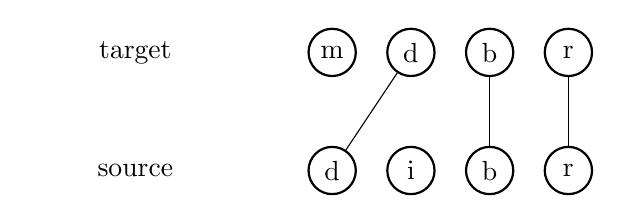
\begin{tikzpicture}[draw=black!100]
 	%[shorten >=1pt,->,draw=black!100]
 	\def \rowtwoht{1.5cm}
 	\def \rowoneht{0.0cm}
 	\tikzstyle{m-node}=[circle,draw=black!100,thick,inner sep=0pt,minimum size=6mm]
 	\tikzstyle{r-node}=[circle,draw=black!100,thick,inner sep=0pt,minimum size=6mm]
 	\tikzstyle{annot} = [text width=2.5cm, text centered]
 	% labels
 	\node[annot] (hidden-label) at (0cm,\rowtwoht) {target};
 	\node[annot] (surface-label) at (0cm,\rowoneht) {source};

 %	\node[annot] (d-label) (0, 0) {observed data vector};
	
 	% hidden layer
 	\node[m-node] 	(m0)	at (2.5cm,\rowtwoht)		{m};
 	\node[m-node] 	(m1)	at (3.5cm,\rowtwoht)		{d};
 	\node[m-node] 	(m2)	at (4.5cm,\rowtwoht)	 	{b};
 	\node[m-node] 	(m3)	at (5.5cm,\rowtwoht) 		{r};
	
 	% surface layer
 	\node[r-node] 	(r0)	at (2.5cm,\rowoneht)		{d};
 	\node[r-node] 	(r1)	at (3.5cm,\rowoneht)		{i};
 	\node[r-node] 	(r2)	at (4.5cm,\rowoneht)	 	{b};
 	\node[r-node] 	(r3)	at (5.5cm,\rowoneht) 		{r};
 	%\node[r-node] 	(r4) 	at (6.5cm,\rowoneht)   		{};
 	%\node[r-node] 	(r5) 	at (7.5cm,\rowoneht)   		{};
	
 	\path (m1)	edge	node	{}	(r0)
 		(m2)	edge	node	{}	(r2)
 		(m3)	edge	node	{}	(r3);
 %		(m3)	edge	node	{}	(r3)
 %		(m1)	edge	node	{}	(r4)
 %		(m3)	edge	node	{}	(r5);
		
 \end{tikzpicture}
 \end{center}
 \caption{The minimum-edit-distance alignment for the Hebrew words \textit{dibr} `he spoke' and \textit{mdbr} `he is speaking'. The discontiguous root \textit{d.b.r} is discovered by aligning \textit{dibr} with \textit{mdbr} and extracting the common subsequence.}
 \label{fig:lev-align}
 \end{mdframed}
 \end{figure}


Other authors simulate a nonlinear, multi-tier representation by 
separating the 
learning process into two or more phases.
The first phase classifies individual literal characters into abstract categories 
that are then 
used by a second phase (and perhaps subsequent phases) to perform other 
aspects of the analysis.
Multiple phases occurring at different times can thus replicate the effects 
of multiple simultaneous levels of representation.
This is the approach taken by \citet{rodrigues-and-cavar:2005} to induce 
the non-concatenative morphology of Arabic. 
%Following the statistical constraint-based method of \cite{elghamry:2005}, 
Their first phase identifies root radicals according to the statistical 
constraint-based method of \citet{elghamry:2005}. 
For each word in their corpus, 
they generate a set of candidate triliteral roots according to 
constraints derived from the tendencies of Arabic roots as observed in corpora. 
In particular, any 3-length subsequence is admitted into the candidate set 
if and only if it satisfies both of the following:
\begin{enumerate} 
\item No two consecutive radicals may be separated by more than two characters.
\item No more than four characters intervene between the first and third radicals.
\end{enumerate}
Then, a statistical score is computed for each candidate, and the one with the highest score is selected as the root.
Once the roots---and thus the stems---have been isolated by the first phase, the second phase identifies the concatenative affixes through a separate methodology.

% Goldsmith and Xanthos
An alternative first-phase strategy can be found in \citet{goldsmith-and-xanthos:2009}, 
who present methods for
partitioning a phonemic inventory into a class of consonants and a class of vowels. 
Their paper does not go into automatic morphological analysis, but it is not difficult to see how C and V classes could be useful to a multi-phase morphological analyzer.
The first phase would partition the phonemic inventory and, for each word, label each phoneme/grapheme as either a consonant or vowel, thus creating a sort of CV skeleton similar to the segmental tier of autosegmental phonology.
Subsequent phases would then use these CV skeletons to isolate roots, patterns, and other morphemes.

While the NSNL approaches described in this section provide a means for detecting discontiguous morphemes, they are not without their weaknesses.
The algorithm of \citet{baroni-et-al:2002} must filter out a large proportion of its input corpus, accepting only the words with relative frequencies of less than 0.01 percent; which are presumed to be content words.
It also relies on arbitrary thresholds; e.g., the threshold for the orthographic similarity measure (defined as $1 - \text{NED}$,  i.e., `$1$ minus the \emph{normalized} minimum edit distance') is set at 0.5, although there is no obvious reason why this should be so.
Note also that behind this threshold is the assumption that morphologically related words share at least half of their characters, which is not necessarily true. Such an assumption would be especially problematic for highly agglutinative languages, 
in which it is not uncommon for a stem to comprise a minority of a word's characters.
Moreover, the Levenshtein edit-distance approach is only capable of comparing words pairwise, which only allows morphological relationships to be expressed on a pairwise basis. This is a consequence of the lack of an explicitly encoded hidden causal layer; an explicit (as opposed to implicit) hidden layer could easily mediate multi-way associations among surface layer components.                                   

% Rodrigues and Cavar
%% Only tri-literal roots
Moreover, \citet{rodrigues-and-cavar:2005}, following \citet{elghamry:2005}, limit their algorithm's search to triliteral roots in order to reduce the problem's complexity, even though quadriliteral roots are not uncommon in Hebrew or Arabic.
%% Reasonable constraints, but constraints nonetheless. A truly general algorithm wouldn't need constraints. 
And while their two constraints on candidate-root generation are quite reasonable, these constraints are particular to the case of Semitic morphology, and thus they would not be required by a truly general algorithm.

Finally, none of the works discussed in this section represents both the hidden layer and surface layer simultaneously in a single, straightforward model. In contrast, the Multiple Cause Mixture Model (MCMM) \citep{saund:94} is an NSNL algorithm that explicitly represents both surface and hidden nodes in a single graphical model. The MCMM is the focus of the next section.

\section{Conclusion}
In sum, both \emph{nonlinearity} and \emph{nonsequentiality} must be present in an algorithm if it is to be handle nonconcatenative morphology. As we have seen through the examples in this chapter, it is not sufficient to have just one of these properties without the other. In the next chapter, we will glean deeper insight into nonlinearity and nonsequentiality by relating them to the mathematical properties of \emph{bipartite} graphs. 